% \documentclass[hidelinks,12pt]{article}
\usepackage[left=0.25cm,top=1cm,right=0.25cm,bottom=1cm]{geometry}
%\usepackage[landscape]{geometry}
\textwidth = 20cm
\hoffset = -1cm
\usepackage[utf8]{inputenc}
\usepackage[spanish,es-tabla]{babel}
\usepackage[autostyle,spanish=mexican]{csquotes}
\usepackage[tbtags]{amsmath}
\usepackage{nccmath}
\usepackage{amsthm}
\usepackage{amssymb}
\usepackage{mathrsfs}
\usepackage{graphicx}
\usepackage{subfig}
\usepackage{standalone}
\usepackage[outdir=./Imagenes/]{epstopdf}
\usepackage{siunitx}
\usepackage{physics}
\usepackage{color}
\usepackage{float}
\usepackage{hyperref}
\usepackage{multicol}
%\usepackage{milista}
\usepackage{anyfontsize}
\usepackage{anysize}
%\usepackage{enumerate}
\usepackage[shortlabels]{enumitem}
\usepackage{capt-of}
\usepackage{bm}
\usepackage{relsize}
\usepackage{placeins}
\usepackage{empheq}
\usepackage{cancel}
\usepackage{wrapfig}
\usepackage[flushleft]{threeparttable}
\usepackage{makecell}
\usepackage{fancyhdr}
\usepackage{tikz}
\usepackage{bigints}
\usepackage{scalerel}
\usepackage{pgfplots}
\usepackage{pdflscape}
\pgfplotsset{compat=1.16}
\spanishdecimal{.}
\renewcommand{\baselinestretch}{1.5} 
\renewcommand\labelenumii{\theenumi.{\arabic{enumii}})}
\newcommand{\ptilde}[1]{\ensuremath{{#1}^{\prime}}}
\newcommand{\stilde}[1]{\ensuremath{{#1}^{\prime \prime}}}
\newcommand{\ttilde}[1]{\ensuremath{{#1}^{\prime \prime \prime}}}
\newcommand{\ntilde}[2]{\ensuremath{{#1}^{(#2)}}}

\newtheorem{defi}{{\it Definición}}[section]
\newtheorem{teo}{{\it Teorema}}[section]
\newtheorem{ejemplo}{{\it Ejemplo}}[section]
\newtheorem{propiedad}{{\it Propiedad}}[section]
\newtheorem{lema}{{\it Lema}}[section]
\newtheorem{cor}{Corolario}
\newtheorem{ejer}{Ejercicio}[section]

\newlist{milista}{enumerate}{2}
\setlist[milista,1]{label=\arabic*)}
\setlist[milista,2]{label=\arabic{milistai}.\arabic*)}
\newlength{\depthofsumsign}
\setlength{\depthofsumsign}{\depthof{$\sum$}}
\newcommand{\nsum}[1][1.4]{% only for \displaystyle
    \mathop{%
        \raisebox
            {-#1\depthofsumsign+1\depthofsumsign}
            {\scalebox
                {#1}
                {$\displaystyle\sum$}%
            }
    }
}
\def\scaleint#1{\vcenter{\hbox{\scaleto[3ex]{\displaystyle\int}{#1}}}}
\def\bs{\mkern-12mu}


% \usepackage{apacite}

\documentclass[12pt]{article}
\usepackage[utf8]{inputenc}
\usepackage[T1]{fontenc}
\usepackage[spanish,es-lcroman]{babel}
\usepackage{amsmath}
\usepackage{amsthm}
\usepackage{amsfonts}
\usepackage{amssymb}
\usepackage{physics}
\AtBeginDocument{\RenewCommandCopy\qty\SI}
\usepackage{tikz}
\usepackage{float}
\usepackage{calc}
\usepackage[autostyle,spanish=mexican]{csquotes}
\usepackage[per-mode=symbol]{siunitx}
\usepackage{textcomp, gensymb}
\usepackage{multicol}
\usepackage{enumitem}
\usepackage{hyperref}
\usepackage{setspace}
\usepackage[left=2.00cm, right=2.00cm, top=2.00cm, 
     bottom=2.00cm]{geometry}
% \usepackage{Estilos/ColoresLatex}
\usepackage{makecell}
\usepackage{subcaption}
\usepackage[skip=10pt, indent=30pt]{parskip}
% \usepackage{scalerel}
\usepackage{scalerel}[2016-12-29]
\usepackage{biblatex}
\usepackage{cancel}

\definecolor{ao}{rgb}{0.0, 0.0, 1.0}
\definecolor{burgundy}{rgb}{0.5, 0.0, 0.13}

\hypersetup{
    colorlinks=true,
    linkcolor=ao,
    filecolor=magenta,      
    urlcolor=ao,
}

\newcommand{\ptilde}[1]{\ensuremath{{#1}^{\prime}}}
\newcommand{\stilde}[1]{\ensuremath{{#1}^{\prime \prime}}}
\newcommand{\ttilde}[1]{\ensuremath{{#1}^{\prime \prime \prime}}}
\newcommand{\ntilde}[2]{\ensuremath{{#1}^{(#2)}}}
\newcommand{\pderivada}[1]{\ensuremath{{#1}^{\prime}}}
\newcommand{\sderivada}[1]{\ensuremath{{#1}^{\prime \prime}}}
\newcommand{\tderivada}[1]{\ensuremath{{#1}^{\prime \prime \prime}}}
\newcommand{\nderivada}[2]{\ensuremath{{#1}^{(#2)}}}

\def\stretchint#1{\vcenter{\hbox{\stretchto[440]{\displaystyle\int}{#1}}}}
\def\scaleint#1{\vcenter{\hbox{\scaleto[3ex]{\displaystyle\int}{#1}}}}
\def\scaleiint#1{\vcenter{\hbox{\scaleto[6ex]{\displaystyle\iint}{#1}}}}
\def\scaleiiint#1{\vcenter{\hbox{\scaleto[6ex]{\displaystyle\iiint}{#1}}}}
\def\scaleoint#1{\vcenter{\hbox{\scaleto[3ex]{\displaystyle\oint}{#1}}}}
\def\bs{\mkern-12mu}

\newcommand{\textocolor}[2]{\textbf{\textcolor{#1}{#2}}}
\sisetup{per-mode=symbol}
\decimalpoint
\sisetup{bracket-numbers = false}
\newlength{\depthofsumsign}
\setlength{\depthofsumsign}{\depthof{$\sum$}}
\newcommand{\nsum}[1][1.4]{% only for \displaystyle
    \mathop{%
        \raisebox
            {-#1\depthofsumsign+1\depthofsumsign}
            {\scalebox
                {#1}
                {$\displaystyle\sum$}%
            }
    }
}

\AtBeginDocument{\RenewCommandCopy\qty\SI}
\ExplSyntaxOn
\msg_redirect_name:nnn { siunitx } { physics-pkg } { none }
\ExplSyntaxOff

\numberwithin{equation}{section}

\linespread{1.15}

\renewcommand{\labelenumii}{\theenumii}
\renewcommand{\theenumii}{\theenumi.\arabic{enumii}.}

\emergencystretch=1em


\title{3 - Construcción de sistemas coordenados especiales \\[0.3em]  \large{Matemáticas Avanzadas de la Física}\vspace{-3ex}}
\author{M. en C. Gustavo Contreras Mayén}
\date{ }

\begin{document}
\vspace{-4cm}
\maketitle
\fontsize{14}{14}\selectfont
\tableofcontents
\newpage

\section{Construcción de sistemas coordenados.}
\subsection{Introducción.}

Una pregunta importante que planteamos en este momento es: ¿para qué estamos revisando los sistemas coordenados curvilíneos?
\par
Como respuesta presentamos la siguiente: Ante un problema de la física, debemos de seleccionar el sistema coordenado de modo que se adapte al problema, \emph{para aprovechar cualquier oportunidad o simetría presente en el mismo}.
\par
De tal manera que resultará más fácil la solución que cuando se obliga a adaptar una solución en un sistema cartesiano.
\par
Cuando se menciona que \enquote{es más fácil la solución}, significa que se tendrá una ecuación diferencial parcial (EDP) que puede separarse en ecuaciones diferenciales ordinarias (EDO), frecuentemente en la \enquote{forma estándar} en el nuevo sistema coordenado.
\par
La \emph{técnica de separación de variables}, se verá en el Tema 2 del curso.

\subsection{Sistemas coordenados especiales.}

Conocemos al menos tres sistemas coordenados con los que hemos trabajado en distintas áreas de nuestra carrera: cartesiano, cilíndrico (en 3D, polar en 2D) y esférico.
\par
De manera conveniente enlistamos catorce sistemas coordenados, que en algún momento nos podremos encontrar.
\par
\textbf{Nota importante: } Debemos de señalar que no es intención de curso que se haga una revisión completa, detallada para cada uno de los sistemas.
\par
Más bien, veremos una metodología con la cual abordaremos el estudio de un sistema coordenado, y entonces tendremos la manera de estudiar otros de acuerdo a las necesidades que se nos presenten.
\par
De manera conveniente se presenta una lista con catorce sistemas, clasificando los mismos de acuerdo con el hecho de que tengan o no:
\begin{enumerate}
\item Un eje de traslación (perpendicular a la familia de superficies de plano paralelo)
\item Un eje de simetría rotacional.
\end{enumerate}

\renewcommand{\arraystretch}{1.2}
\begin{table}[H]
\centering
\begin{tabular}{p{4cm} p{6cm} p{4cm}}
Eje de traslación & Eje de rotación & Ninguno \\ \hline
Cartesiano ($3$ ejes) & & Confocal elipsoidal \\
Circular cilíndrico & Circular cilíndrico & \\
& Polar esferoidal ($3$ ejes) & \\
Elíptico cilíndrico & Esferoidal prolato o alargado & \\
& Esferoidal oblato & \\
Parabólico cilíndrico & Parabólico & \\
Bipolar & Toroidal & \\
& Biesférico & \\[0.5em]
& & Cónico \\
& & Confocal paraboidal \\
\end{tabular}
\caption{Tabla con distintos sistemas coordenados.}
\label{table:tabla_01}
\end{table}

El espaciamiento en la tabla (\ref{table:tabla_01}) indica las relaciones entre los diversos sistemas coordenados.
\par
Si se considera el caso en dos dimensiones ($z = 0$) de un sistema con un eje de traslación (columna izquierda) y se le hace girar alrededor de un eje de simetría de reflexión, se genera el sistema coordenado correspondiente indicado en la columna central hacia la derecha.
\par
Por ejemplo: la rotación del plano $z = 0$ del sistema cilíndrico elíptico alrededor del eje principal genera el sistema esferoidal alargado; la rotación alrededor del eje menor resulta en el sistema esferoidal oblato.
\par
También se consideran tres sistemas que no tienen eje de traslación o eje de rotación. En este grupo asimétrico, el sistema elipsoidal confocal se utiliza algunas veces como el sistema más general y del que casi todos los demás sistemas se obtienen del mismo.

\section{Desarrollo de un sistema coordenado.}

\subsection{Coord. cilíndricas elípticas \texorpdfstring{$(u, v, z)$}{(u, v, z)}.}

A continuación veremos la manera de abordar un sistema coordenado especial, para determinar los las superficies constantes, los factores de escala, los operadores diferenciales, necesarios para resolver un problema con esta geometría en particular.

\subsection{Reglas de transformación.}

Para el sistema cilíndrico elíptico, se tienen las siguientes reglas de transformación:
\begin{align}
\begin{aligned}
    (x, y, z) &\Rightarrow (u, v, z) \\
x &= a \, \cosh u \, \cos v \\
y &= a \, \sinh u \, \sin v \\
z &= z
\end{aligned}
\label{eq:ecuacion_02_73_esp}
\end{align}

\subsection{Superficies coordenadas.}

Para identificar las superficies constantes, elevamos al cuadrado cada lado:
\begin{align}
x^{2} &= a^{2} \, \cosh^{2} u \, \cos^{2} v \label{eq:ecuacion_02_74_esp} \\
y^{2} &= a^{2} \, \sinh^{2} u \, \sin^{2} v \label{eq:ecuacion_02_75_esp}
\end{align}

Dividimos la primera expresión entre $\cos^{2} v$:
\begin{align*}
\dfrac{x^{2}}{\cos^{2} v} &= \dfrac{a^{2} \, \cosh^{2} u \, \cos^{2} v}{\cos^{2} v} \\[0.5em]
\dfrac{x^{2}}{\cos^{2} v} &= a^{2} \, \cosh^{2} u \\[0.5em]
\Rightarrow \hspace{0.3cm} \dfrac{x^{2}}{a^{2} \, \cosh^{2} u} &= \cos^{2} v 
\end{align*}

y la segunda entre $\sin^{2} v$:
\begin{align*}
\dfrac{y^{2}}{\sin^{2} v} &= \dfrac{a^{2} \, \sinh^{2} u \, \sin^{2} v}{\sin^{2} v} = a^{2} \, \sinh^{2} u  \\[0.5em]
\Rightarrow \hspace{0.3cm} \dfrac{y^{2}}{a^{2} \, \sinh^{2} u} &= \sin^{2} v
\end{align*}
recordando que:
\begin{align*}
\cos^{2} v + \sin^{2} v = 1 \\[0.5em]
\cosh^{2} u - \sinh^{2} u = 1
\end{align*}
así llegamos a:
\begin{align}
\dfrac{x^{2}}{a^{2} \, \cosh^{2}} + \dfrac{y^{2}}{a^{2} \, \sinh{2}} &= \cos^{2} + \sin^{2} = 1 \label{eq:ecuacion_02_76_esp}\\[1em]
\dfrac{x^{2}}{a^{2} \, \cos^{2}} - \dfrac{y^{2}}{a^{2} \, \sin^{2}} &= \cosh^{2} - \sinh^{2} = 1 \label{eq:ecuacion_02_77_esp}
\end{align}

Para $v=$ constante, la ec. (\ref{eq:ecuacion_02_76_esp}) genera una familia de elipses con el eje $x$, en el principal.
\par
Para $u=$ constante, la ec. (\ref{eq:ecuacion_02_77_esp}) genera hipérbolas con puntos focales en el eje $x$. Como se pueden ver en la siguiente figura (\ref{fig:figura_coordenada_cilindricas_elipticas})

\begin{figure}[H]
    \centering
    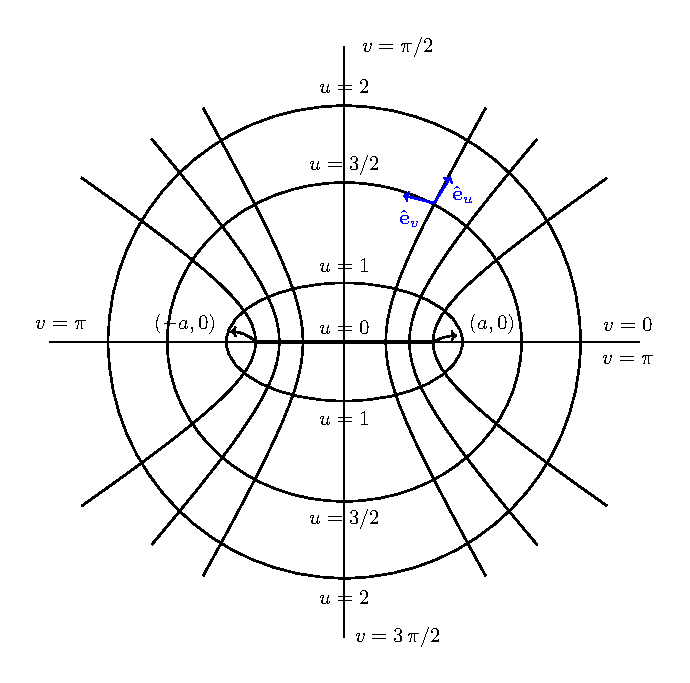
\includegraphics[scale=1]{Imagenes/Sistema_Cilindrico_Eliptico.eps}
    \caption{Sistema coordenado cilíndrico elíptico en el plano $x-y$.}
    \label{fig:figura_coordenada_cilindricas_elipticas}
\end{figure}
Por último, para $z$ constante, tenemos una familia de planos en $x - y$.

La familia de superficies coordenadas son las siguientes:
\begin{enumerate}
\item Cilindros elípticos con $u$ constante, $0 \leq u < \infty$
\item Cilindros hiperbólicos con $v$ constante, $0 \leq v \leq 2 \, \pi$
\item Planos paralelos al plano $x-y$ con $z$ constante, $-\infty < z < \infty$
\end{enumerate}
Como vemos en la siguiente figura (\ref{fig:figura_coordenada_cilindricas_elipticas_3D}):

\begin{figure}[H]
    \centering
    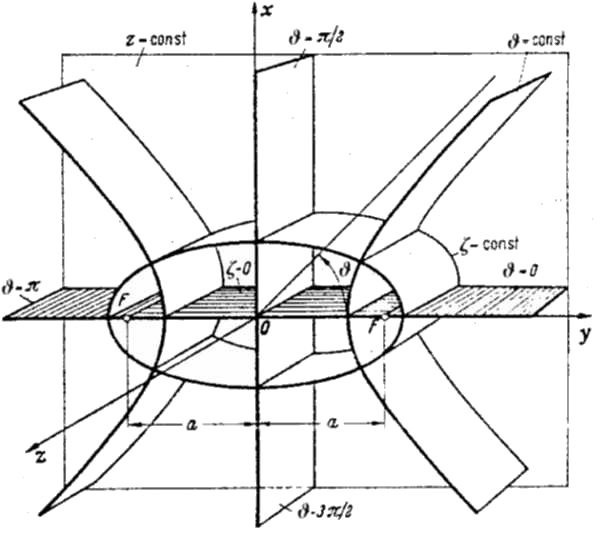
\includegraphics[scale=0.6]{Imagenes/Elliptic-cylindrical-coordinates_02.png}
    \caption{Sistema coordenado cilíndrico elíptico en una vista 3D.}
    \label{fig:figura_coordenada_cilindricas_elipticas_3D}
\end{figure}

\subsection{Factores de escala.}

Calculamos los factores de escala o coeficientes métricos a partir de la expresión:
\begin{align*}
h_{i} &= \abs{\pdv{\vb{r}}{u_{i}}} \\[0.5em]
h_{i} &= \sqrt{ \left( \pdv{x}{u_{i}} \right)^{2} + \left( \pdv{y}{u_{i}} \right)^{2} + \left( \pdv{z}{u_{i}} \right)^{2}}
\end{align*}

Tenemos entonces que:
\begin{align*}
h_{1} = h_{u} = \sqrt{ \left( \pdv{x}{u} \right)^{2} + \left( \pdv{y}{u} \right)^{2} + \left( \pdv{z}{u} \right)^{2}}
\end{align*}
donde las derivadas parciales son:
\begin{align*}
\pdv{x}{u} &= a \, \sinh u \cos v \hspace{0.5cm} \Rightarrow \hspace{0.5cm} \left( \pdv{x}{u} \right)^{2} = a^{2} \, \sinh^{2} u \, \cos^{2} v \\[0.5em]
\pdv{y}{u} &= a \, \cosh u \sin v \hspace{0.5cm} \Rightarrow \hspace{0.5cm} \left( \pdv{y}{u} \right)^{2} = a^{2} \, \cosh^{2} u \, \sin^{2} v \\[0.5em]
\pdv{z}{u} &= 0
\end{align*}
\\[0.5em]
Al sumar los términos del radical:
\begin{align*}
h_{u} = \sqrt{a^{2} \, \sinh^{2} u \, \cos^{2} v + a^{2} \, \cosh^{2} u \, \sin^{2} v}
\end{align*}
\\[0.5em]
Haciendo el álgebra respectiva y considerando que $\cosh^{2} u - \sinh^{2} = 1$, entonces tenemos que:
\begin{align*}
h_{u} &= \sqrt{a^{2} \left[ \sinh^{2} u \, \cos^{2} v + \cosh^{2} u \, \sin^{2} v \right] } \\[0.5em]
&= \sqrt{a^{2} \left[ \sinh^{2} u \, \cos^{2} v + (1 + \sinh^{2} u) \, \sin^{2} v \right] } \\[0.5em]
&= \sqrt{a^{2} \left[ \sinh^{2} u \, \cos^{2} v + \sinh^{2} u \, \sin^{2} v + \sin^{2} v \right] } \\[0.5em]
&= \sqrt{a^{2} \left[ \sinh^{2} u ( \cos^{2} v + \sin^{2} v ) + \sin^{2} v \right] } \\[0.5em]
&= \sqrt{a^{2} \left[ \sinh^{2} u + \sin^{2} v  \right] }
\end{align*}
\begin{equation*}
\hspace{-4.5cm} \boxed{ h_{u} = a \, \sqrt{ \sinh^{2} u + \sin^{2} v}}
\end{equation*}
\\[0.5em]
Para el factor $h_{v}$ se tiene que:
\begin{align*}
h_{v} = \sqrt{ \left( \pdv{x}{v} \right)^{2} + \left( \pdv{y}{v} \right)^{2} + \left( \pdv{z}{v} \right)^{2}}
\end{align*}
\\[0.5em]
Entonces:
\begin{align*}
\pdv{x}{v} &= - a \, \cosh u \sin v \hspace{0.5cm} \Rightarrow \hspace{0.5cm} \left( \pdv{x}{v} \right)^{2} = a^{2} \, \cosh^{2} u \, \sin^{2} v \\[0.5em]
\pdv{y}{v} &= a \, \sinh u \cos v \hspace{0.5cm} \Rightarrow \hspace{0.5cm} \left( \pdv{y}{v} \right)^{2} = a^{2} \, \sinh^{2} u \, \cos^{2} v \\[0.5em]
\pdv{z}{v} &= 0
\end{align*}
\\[0.5em]
Así llegamos a:
\begin{align*}
h_{v} &= \sqrt{a^{2} \left[ \cosh^{2} u \, \sin^{2} v + \sinh^{2} u \, \cos^{2} v \right] } \\[0.5em]
&= \sqrt{a^{2} \left[ (1 + \sinh^{2} u) \, \sin^{2} v + \sinh^{2} u \, \cos^{2} v \right] } \\[0.5em]
&= \sqrt{a^{2} \left[ \sinh^{2} u (\cos^{2} v +  \sin^{2} v)+ \sin^{2} v \right] } \\[0.5em]
&= \sqrt{a^{2} \left[ \sinh^{2} u + \sin^{2} v  \right] }
\end{align*}
\begin{equation*}
\hspace{-4.5cm}
\boxed{h_{v} = a \, \sqrt{ \sinh^{2} u + \sin^{2} v}}
\end{equation*}
\\[0.5em]
Para el último factor de escala $h_{z}$:
\begin{align*}
h_{z} = \sqrt{ \cancelto{0}{\left( \pdv{x}{z} \right)^{2}} + \cancelto{0}{\left( \pdv{y}{z} \right)^{2}} + \cancelto{1}{\left( \pdv{z}{z} \right)^{2}}}
\end{align*}
\begin{equation*}
\hspace{-4.5cm} \boxed{h_{z} = 1}
\end{equation*}
\\[0.5em]
Los tres factores de escala para este sistema coordenado cilíndrico elíptico son:
\begin{align*}
h_{u} &= a \, \sqrt{ \sinh^{2} u + \sin^{2} v} \\[1em]
h_{v} &= a \, \sqrt{ \sinh^{2} u + \sin^{2} v} \\[1em]
h_{z} &= 1
\end{align*}
% \\[0.5em]
% \noindent
% \textbf{Ejercicio a cuenta (11). } Para el sistema de coordenadas esferoidales prolatas $(\xi, \eta, \phi)$, cuyas reglas de transformación son:
% \begin{align*}
% x &= a \: \sinh \xi \: \sin \eta \: \cos \phi\\
% y &= a \: \sinh \xi \: \sin \eta \: \sin \phi\\
% z &= a \: \cosh \xi \: \cos \eta
% \end{align*}
% \begin{enumerate}
% \item Describe las superficies coordenadas del sistema.
% \item Calcula de manera explícita los factores de escala $(h_{\xi}, h_{\eta}, h_{\phi})$.
% \end{enumerate}
% Nota: aunque más adelante se indica cuáles son los factores de escala, deberás de realizar todo el procedimiento para el cálculo de los mismos, y podrás corroborar tus resultados con esos valores.

\section{Cálculo de los operadores diferenciales.}

\subsection{Gradiente.}

Ya definimos una expresión que nos permitirá calcular el gradiente sobre una función de prueba $\phi$, una vez conocidos los factores de escala del sistema coordenado de interés:
\begin{align*}
\nabla{\phi} = \sum_{i=1}^{3} \dfrac{\vu{e_{i}}}{h_{i}} \, \pdv{\phi}{u_{i}} = \sum_{i=1}^{3} \vu{e}_{i} \left( \nabla{\phi} \right)_{i}
\end{align*}
Por lo que: 
\begin{align*}
\grad{\phi} &= \sum_{i=1}^{3} \dfrac{\vu{e_{i}}}{h_{i}} \, \pdv{\phi}{u_{i}}
\end{align*}
Entonces:
\begin{align*}
\grad{\phi} = \dfrac{1}{a \sqrt{\sinh^{2} u + \sin^{2} v}} \left[ \vu{e}_{u} \pdv{\phi}{u} + \vu{e}_{v} \pdv{\phi}{v} \right] + \vu{e_{z}} \pdv{\phi}{z}
\end{align*}

\subsection{Divergencia.}

Para un campo vectorial $\vb{B}$, habíamos llegado al resultado:
\begin{align*}
\div{\vb{B}} = \dfrac{1}{h} \, \sum_{i=1}^{3} \pdv{u_{i}} \left( \dfrac{B_{i} \, h}{h_{i}} \right)
\end{align*}
donde $h = h_{1} h_{2} h_{3}$, así entonces:
\begin{align*}
\div{\vb{B}} &= \dfrac{1}{h} \left[ \pdv{u} \left( B_{u} \, h_{2} \, h_{3} \right) + \pdv{v} \left( B_{v} \, h_{1} \, h_{3} \right) + \pdv{z} \left( B_{z} \, h_{1} \, h_{2} \right) \right]
\end{align*}
Al realizar las respectivas operaciones y reduciendo las expresiones (tarea moral que puedes hacer), haciendo $h^{\prime} = \sqrt{\sinh^{2} u + \sin^{2} v}$, tenemos que:
\begin{align*}
\div{\vb{B}} &= \dfrac{1}{a \, h^{\prime}} \left[ \pdv{u} \left( h^{\prime} \, B_{u} \right) + \pdv{v} \left( h^{\prime} \, B_{v} \right) \right] + \pdv{B_{z}}{z}
\end{align*}

\subsection{Cálculo del rotacional.}

Para calcular el rotacional de un campo vectorial, ocupamos la expresión:
\begin{align*}
\curl{\vb{B}} = \dfrac{1}{h_{1} h_{2} h_{3}} \, \mdet{
h_{1} \, \vu{e}_{1} & h_{2} \, \vu{e}_{2} & h_{3} \, \vu{e}_{3} \\
\displaystyle \pdv{u_{1}} & \displaystyle \pdv{u_{2}} & \displaystyle \pdv{u_{3}} \\
B_{1} \, h_{1} & B_{2} \, h_{2} & B_{3} \, h_{3}
}
\end{align*}
Entonces tendremos que:
\begin{align*}
\curl{\vb{B}} &= \dfrac{\vu{e}_{u}}{h_{v} h_{z}} \left[ \displaystyle \pdv{v} \left( B_{z} \, h_{z} \right) - \pdv{z} \left( B_{v} \, h_{v} \right) \right] + \\[0.5em]
&+ \dfrac{\vu{e}_{v}}{h_{z} h_{u}} \left[ \displaystyle \pdv{u_{z}} \left( B_{u} \, h_{u} \right) - \pdv{u} \left( B_{z} \, h_{z} \right) \right] + \\[0.5em]
&+ \dfrac{\vu{e}_{z}}{h_{u} h_{v}} \left[ \displaystyle \pdv{u} \left( B_{v} \, h_{v} \right) - \pdv{v} \left( B_{u} \, h_{u} \right) \right]
\end{align*}
Calculamos las correspondientes derivadas parciales, multiplicamos los factores de escala, para luego  simplificar la expresión y presentarla en términos de un determinante.

Entonces haciendo $h^{\prime} = \sqrt{\sinh^{2} u + \sin^{2} v}$, llegamos a:
\begin{align*}
\curl{\vb{B}} &= \dfrac{1}{h^{\prime 2}} \, \mdet{
h^{\prime} \, \vu{e}_{u} & h^{\prime} \, \vu{e}_{v} & \vu{e}_{z} / a \\[0.5em]
\displaystyle \pdv{u_{u}} & \displaystyle \pdv{u_{v}} & \displaystyle \pdv{u_{z}} \\[1em]
B_{u} \, h^{\prime} & B_{v} \, h^{\prime} & B_{z} / a
}
\end{align*}
Queda también como tarea moral hacer el desarrollo de cada oepración y corroborar el resultado.

\subsection{Laplaciano.}

Para una función escalar $\phi$, definimos el Laplaciano como:
\begin{align*}
\laplacian{\phi} = \dfrac{1}{h} \, \sum_{i=1}^{3} \pdv{u_{i}} \left( \dfrac{h}{h_{i}^{2}}  \pdv{\phi}{u_{i}} \right)
\end{align*}
con $h = h_{1} h_{2} h_{3}$.
\par
Así pues, tenemos que:
\begin{align*}
\laplacian{\phi} = \dfrac{1}{a^{2} \left( \sinh^{2} u + \sin^{2} v \right)} \left[ \pdv[2]{\phi}{u} + \pdv[2]{\phi}{v} \right] + \pdv[2]{\phi}{z}
\end{align*}


\section{Más sistemas coordenados.}

\subsection{Algunos sistemas.}

Al comenzar el Tema 1, se mencionó que durante nuestra formación como físicos, hemos trabajado de manera natural en al menos $3$ sistemas coordenados: cartesiano, cilíndrico y esférico.
\par
Sin embargo, hay que tener en cuenta que existen otros sistemas coordenados, cada uno de ellos con sus respectivas reglas de transformación.
\par
La revisión y procedimiento que hemos hecho con el sistema de coordenadas cilíndricas elípticas, para obtener los factores de escala así como los operadores diferenciales, es la guía con la cual podemos obtener los correspondientes de estos otros sistemas.
\par
Sería un muy buen ejercicio moral, el que obtengas esos valores y construyas una tabla.
\par
Es cierto que puedes consultarlos en algunos textos de física matemática, pero la práctica con el trabajo a mano, nos ayuda bastante para tener presente la secuencia de pasos, además de reforzar nuestras habilidades de razonamiento matemático.

\subsection{Solución de una ecuación.}

En este Tema 1 que nos refiere a la física y a la geometría, es un buen punto de partida para plantear el tema de dar solución a una ecuación bajo un nuevo sistema coordenado.
\par
La ecuación de Helmholtz:
\begin{align}
\nabla^{2} \psi + k^{2} \: \psi = 0
\label{eq:ecuacion_02_01}
\end{align}
es una ecuación separable.
\par
Es decir, podemos reexpresar esta ecuación en un sistema coordenado distinto.
\par
En particular ésta ecuación tiene el hecho de que si:
\begin{itemize}
\item $k^{2} = 0$, se obtiene la ecuación de Laplace.
\item $k^{2} = (+) \mbox{ constante}$, se obtiene la ecuación de Helmholtz.
\item $k^{2} = (-) \mbox{ constante}$, se obtiene la ecuación de difusión (en su parte espacial).
\item $k^{2} = \mbox{ constante } \times \mbox{ energía cinética}$, se obtiene la ecuación de onda de Schrödinger.
\end{itemize}

Se ha demostrado que existen once sistemas coordenados en donde la ec. de Helmholtz puede separarse. 
\par
Naturalmente, hay un costo que se debemos pagar por el uso de un sistema diferente al de coordenadas cartesianas.
\par
En este punto del Tema 1, ya podemos \enquote{pagar} ese costo por el cambio de un sistema coordenado distinto, y sería también una tarea moral que logres revisar sino en todos los sistemas que mostraremos a continuación, al menos en unos $5$ sistemas.
\par
\textbf{Importante: } Cabe señalar que en algunos textos se ocupa una notación para las nuevas coordenadas con letras del alfabeto castellano: $(u,v,w)$.
\par
Otros textos ocupan letras griegas: $(\xi, \eta, \mu, \nu, \theta, \psi, \phi)$.
\par
Sin pérdida de generalidad, ocupar cualquiera de las notaciones indicadas representa lo mismo. Lo importante es trabajar con las reglas de transformación.
\par
A continuación presentaremos algunos sistemas coordenados: el dominio de las coordenadas, las reglas de transformación, los factores de escala y un representación visual de las superficies.

\section{Otros \texorpdfstring{$11$}{11} sistemas coordenados.}

En el siguiente desarrollo se presentan las reglas de transformación para distintos sistemas coordenados, así como un bosquejo de las superficies coordenadas y de manera explícita los factores de escala. En caso que se pida resolver un ejercicio que involucre a alguno de los sistemas mencionados, se deberá de realizar la correspondiente explicación ya sea para las superficies coordenadas o con los factores de escala, este material les servirá de consulta para corroborar sus resultados.

\subsection{Coord. cilíndricas parabólicas \texorpdfstring{$(u, v, z)$}{(u, v, z)}.}

\begin{minipage}{0.45\textwidth}
Dominio de las coordenadas:
\begin{align*}
u &\in (-\infty,\infty) \\
v &\in [0,\infty) \\
z &\in(-\infty,\infty)
\end{align*}
\end{minipage}
\hspace{1cm}
\begin{minipage}{0.4\textwidth}
Reglas de transformación:
\begin{align*}
x &= \dfrac{1}{2}(u^{2 } -v^{2}) \\
y &= u \: v \\
z &=z
\end{align*}
\end{minipage}
\\[0.75em]
Factores de escala:
\begin{align*}
h_{1 } &= h_{2} = \sqrt{u^{2 } +v^{2}} \\
h_{3 } &= 1
\end{align*}

\begin{figure}[H]
  \centering
  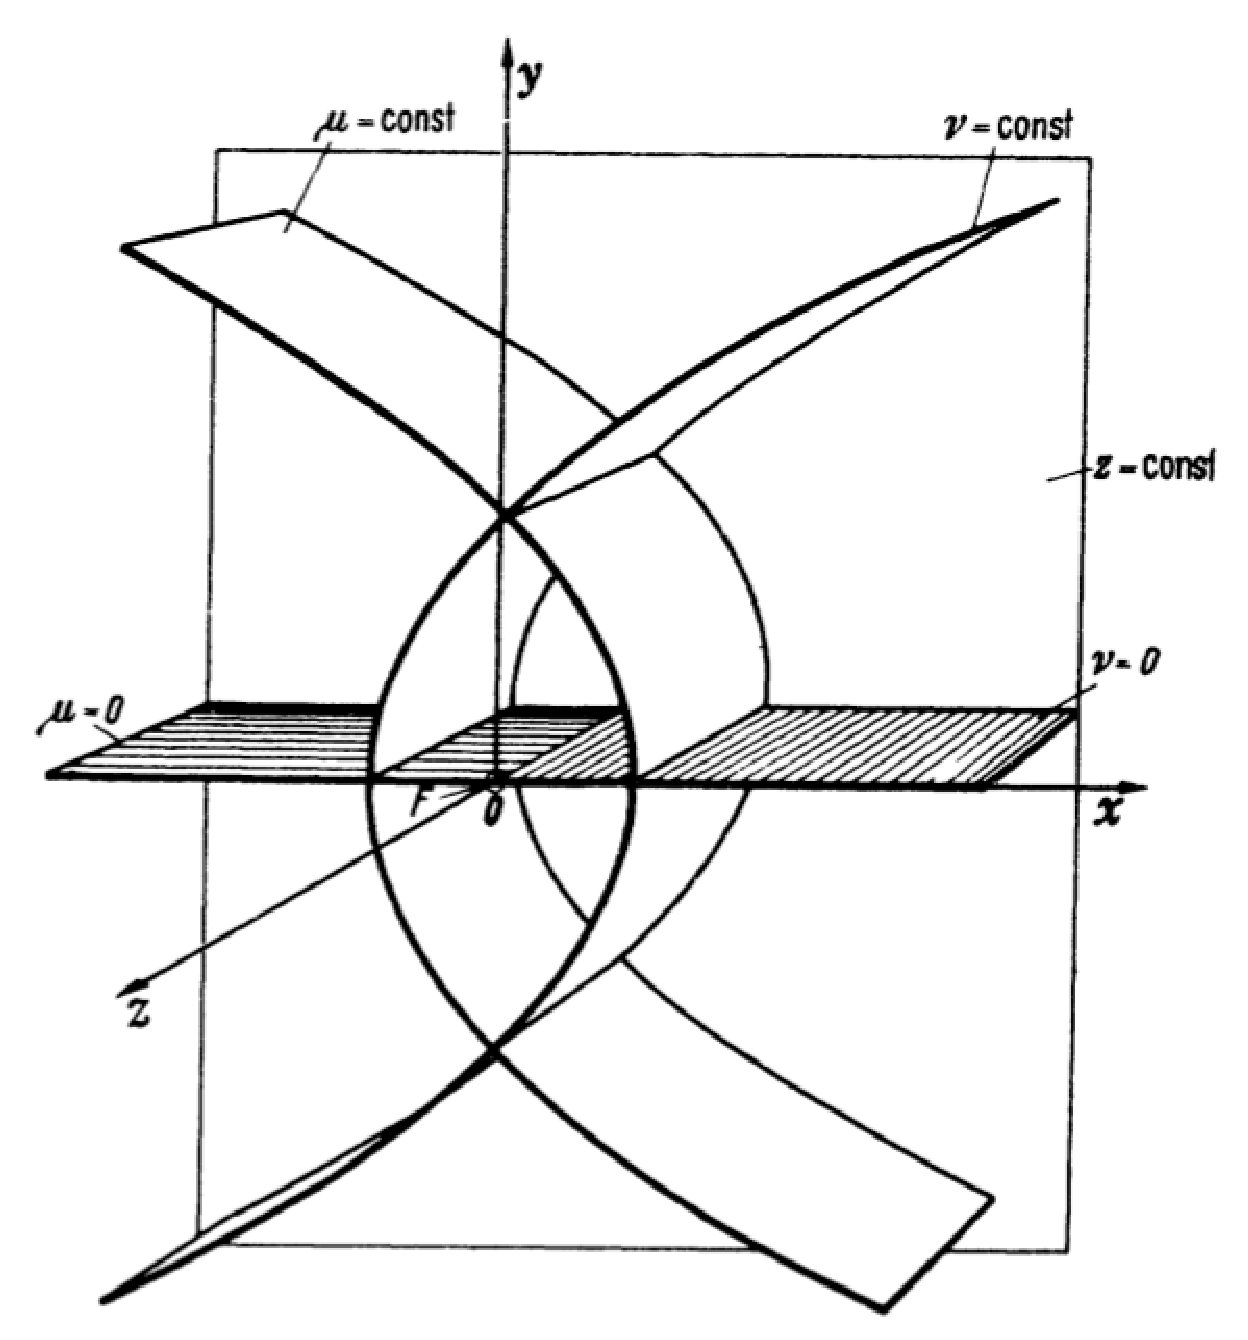
\includegraphics[scale=0.5]{Imagenes/Sistema_Cilindrico_Parabolico.eps}
  \caption{Sistema coordenado cilíndrico parabólico.}
\end{figure}

\subsection{Coord. esferoidales prolatas \texorpdfstring{$(\xi, \eta, \phi)$}{x,e,f}.}

\begin{minipage}{0.45\textwidth}
Dominio de las coordenadas:
\begin{align*}
\xi &\in [0, \infty) \\
\eta &\in [0, \pi] \\
\phi &\in [0, 2 \: \pi)
\end{align*}
\end{minipage}
\hspace{1cm}
\begin{minipage}{0.4\textwidth}
Reglas de transformación:
\begin{align*}
x &= a \: \sinh \xi \: \sin \eta \: \cos \phi\\
y &= a \: \sinh \xi \: \sin \eta \: \sin \phi\\
z &= a \: \cosh \xi \: \cos \eta
\end{align*}
\end{minipage}
\\[0.75em]
Factores de escala:
\begin{align*}
h_{1} &= h_{2} = a \: \sqrt{\sinh^{2} \xi + \sin^{2} \eta} \\
h_{3 }&= a \: \sinh \xi \: \sin \eta
\end{align*}

\begin{figure}[H]
  \centering
  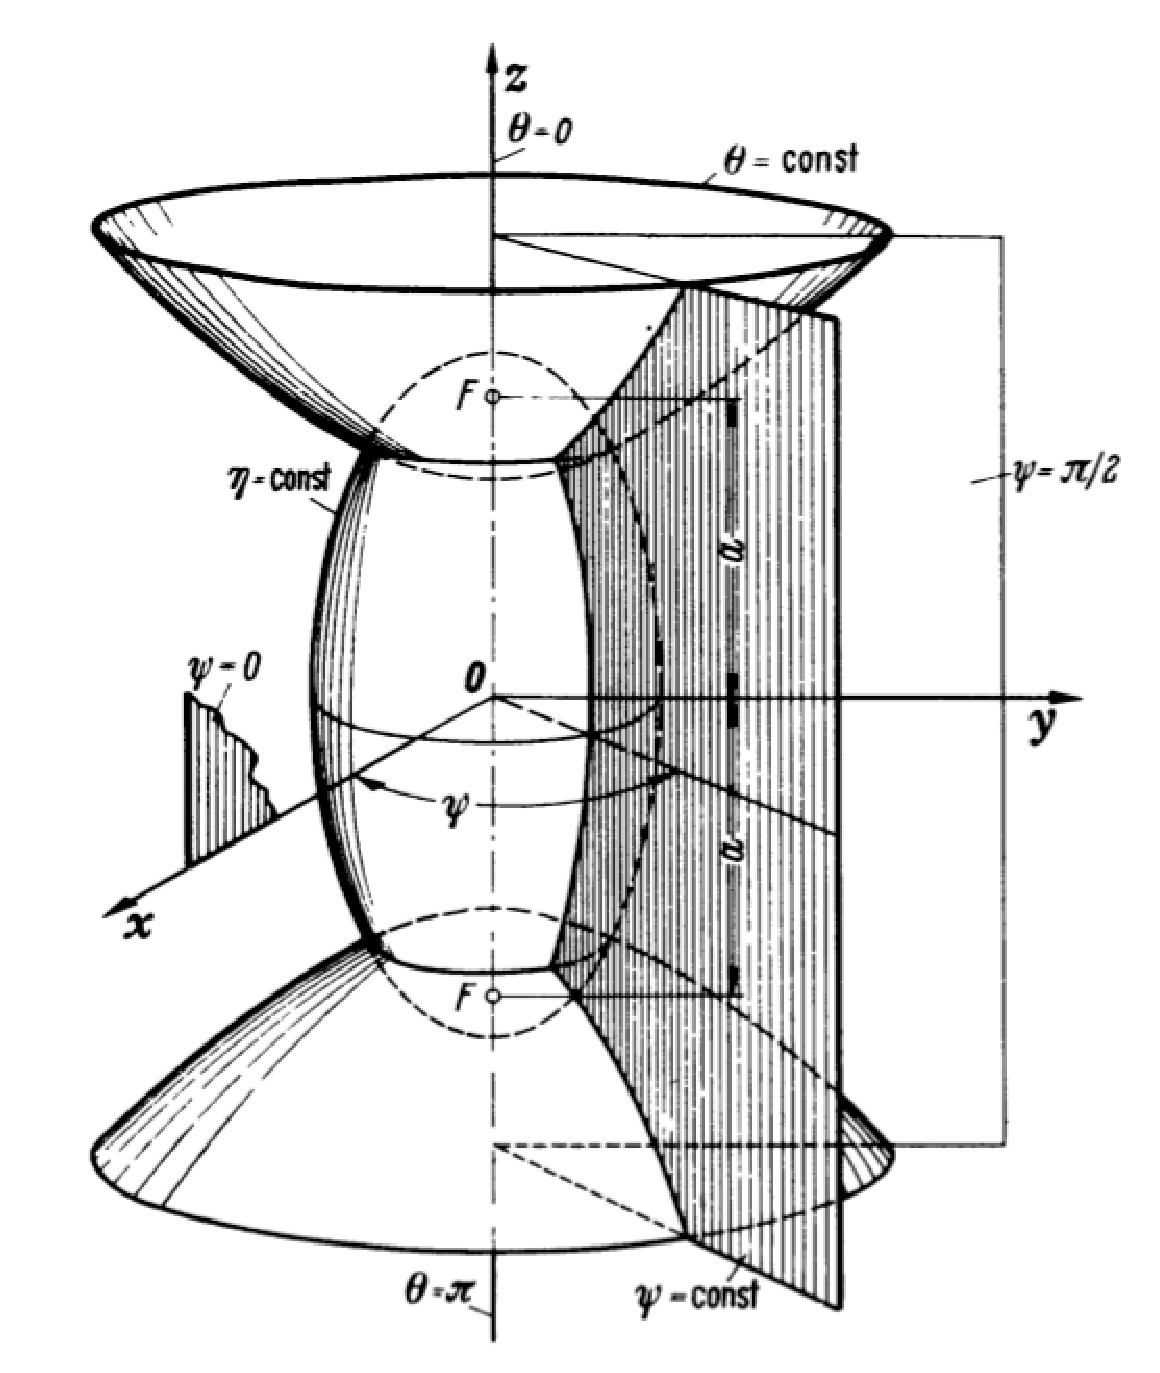
\includegraphics[scale=0.5]{Imagenes/Sistema_Esfeoridal_Prolato.eps}
  \caption{Sistema coordenado esferoidal prolato.}
\end{figure}

\subsection{Coord. esferoidales oblatas \texorpdfstring{$(\xi, \eta, \phi)$}{(x,e, f)}.}

\begin{minipage}{0.45\textwidth}
Dominio de las coordenadas:
\begin{align*}
\xi &\in [0, \infty) \\
\eta &\in \left[- \dfrac{\pi}{2}, \dfrac{\pi}{2} \right] \\
\phi &\in [0, 2\: \pi)
\end{align*}
\end{minipage}
\hspace{1cm}
\begin{minipage}{0.4\textwidth}
Reglas de transformación:
\begin{align*}
x &= a \: \cosh \xi \: \cos \eta \: \cos \phi \\
y &= a \: \cosh \xi \: \cos \eta \: \sin \phi\\
z &= a \: \sinh \xi \: \sin \eta
\end{align*}
\end{minipage}
\\[0.75em]
Factores de escala:
\begin{align*}
h_{1 }&= h_{2} = a \: \sqrt{\sinh^{2} \xi + \sin^{2} \eta} \\
h_{3 }&= a \: \cosh \xi \: \cos \eta
\end{align*}

\begin{figure}[H]
  \centering
  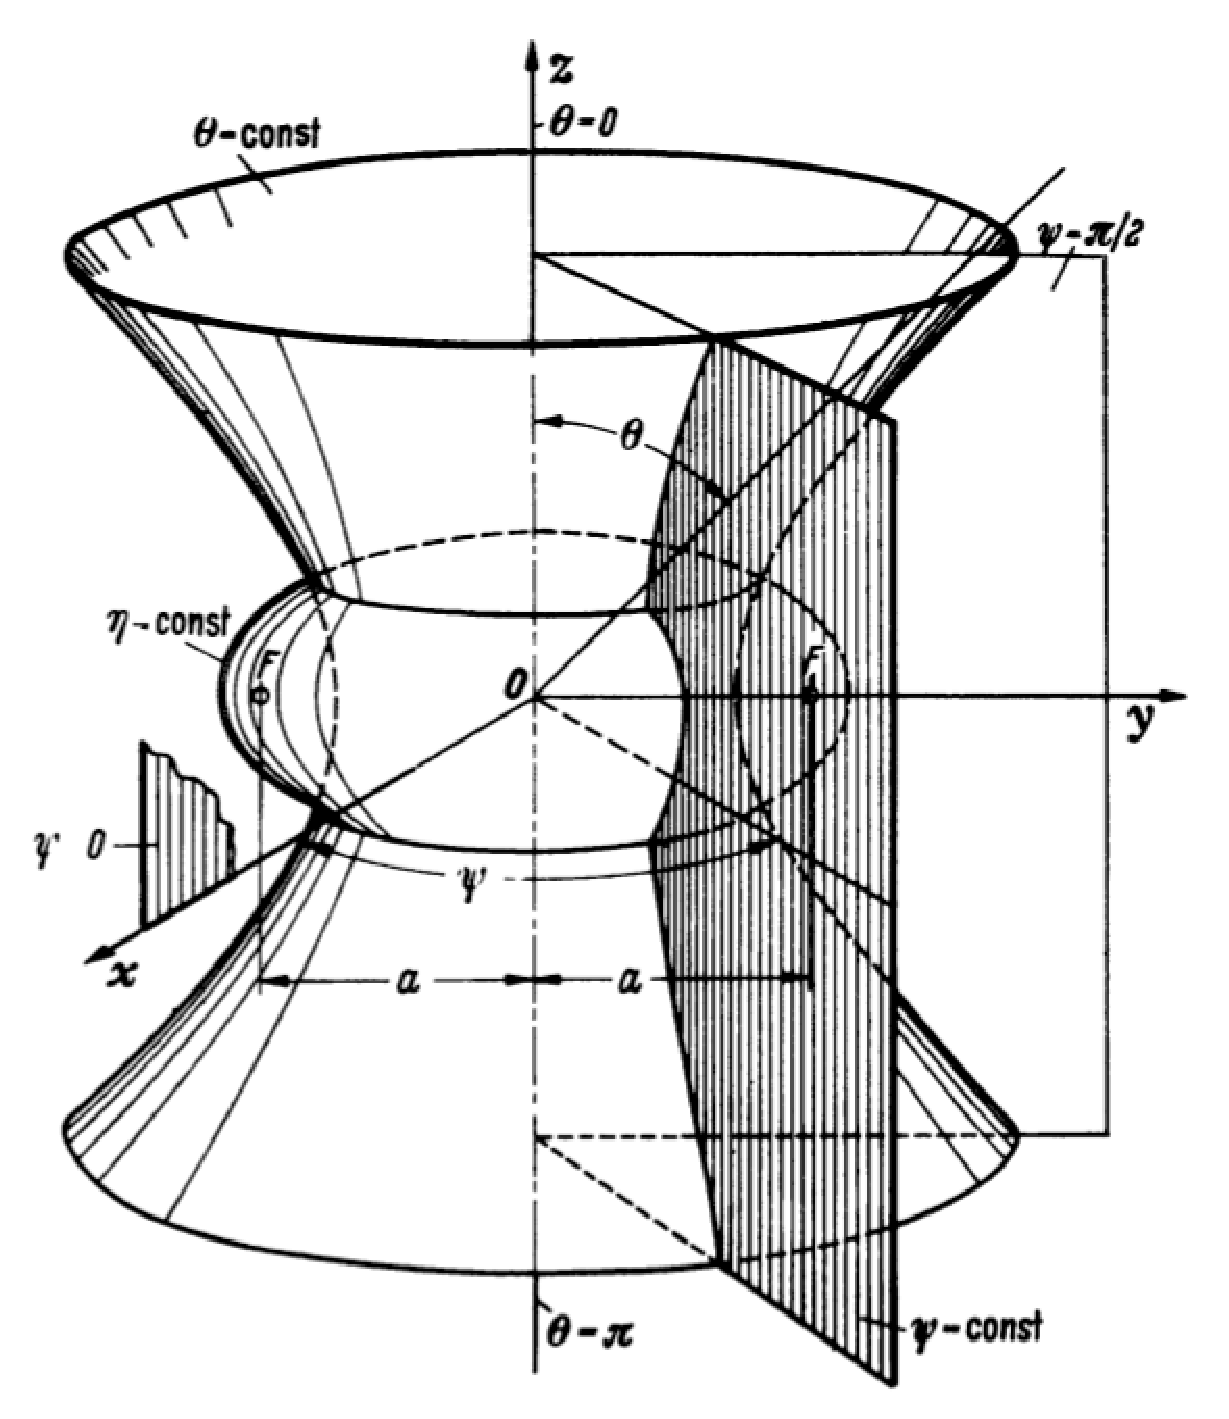
\includegraphics[scale=0.5]{Imagenes/Sistema_Esfeoridal_Oblato.eps}
  \caption{Sistema coordenado esferoidal oblato.}
\end{figure}

\subsection{Coord. parabólicas \texorpdfstring{$(u, v, \phi)$}{(u, v, f)}.}

\begin{minipage}{0.4\textwidth}
Dominio de las coordenadas:
\begin{align*}
u &\in [0, \infty) \\
v &\in [0, \infty) \\
\phi &\in [0, 2 \: \pi)
\end{align*}
\end{minipage}
\hspace{1cm}
\begin{minipage}{0.4\textwidth}
Reglas de transformación:
\begin{align*}
x &= u \: v \: \cos \phi \\
y &= u \: v \: \sin \phi \\
z &= \dfrac{1}{2} (u^{2} - v^{2})
\end{align*}
\end{minipage}

Factores de escala:
\begin{align*}
h_{1} &= h_{2} = \sqrt{u^{2 } +v^{2}} \\
h_{3} &= u \: v
\end{align*}

\begin{figure}[H]
    \centering
    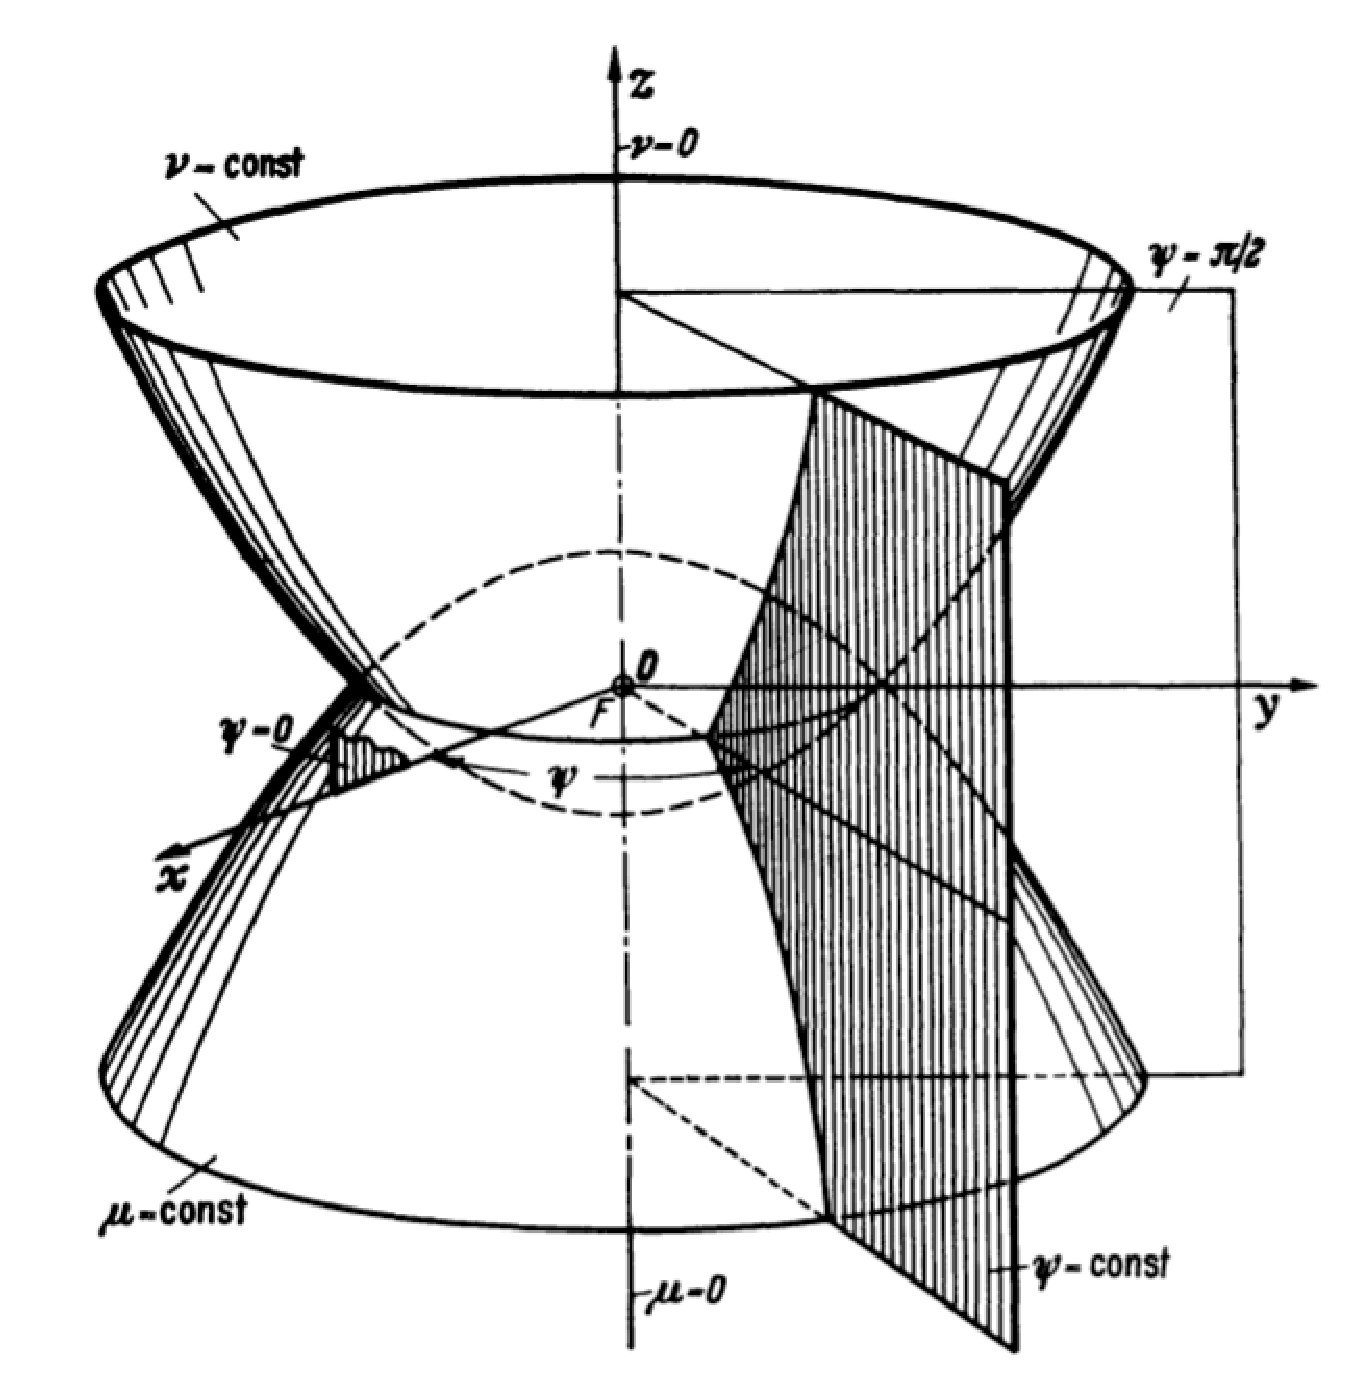
\includegraphics[scale=0.5]{Imagenes/Sistema_Parabolico.eps}
    \caption{Sistema coordenado parabólico.}
\end{figure}

\subsection{Coord. cónicas \texorpdfstring{$(r, \theta, \lambda)$}{(r, t, l)}.}

Dominio de las coordenadas:
\begin{align*}
0 &\leq r < \infty \\
b^{2} &< \theta < c^{2} \\
0 &< \lambda^{2} < b^{2}
\end{align*}
Con:
\begin{align*}
c^{2} > \theta^{2} > b^{2} > \lambda^{2} > 0
\end{align*}

Reglas de transformación:
\begin{align*}
(x)^{2} &= \left( \dfrac{r \, \theta \, \lambda}{b \, c} \right)^{2} \\[0.5em]
(y)^{2} &= \dfrac{r^{2} (\theta^{2} - b^{2})(b^{2} - \lambda^{2})}{b^{2}(c^{2} - b^{2})} \\[0.5em]
(z)^{2} &= \dfrac{r^{2} (c^{2} - \theta^{2})(c^{2} - \lambda^{2})}{c^{2} (c^{2} - b^{2})}
\end{align*}

Factores de escala:
\begin{align*}
h_{1} &= 1\\
(h_{2})^{2} &= \dfrac{r^{2} (\theta^{2} - \lambda^{2})}{(\theta^{2} - b^{2})(c^{2} - \theta^{2})} \\[0.5em]
(h_{3})^{2} &= \dfrac{r^{2} (\theta^{2} - \lambda^{2})}{(b^{2} - \lambda^{2})(c^{2} - \lambda^{2})}
\end{align*}

\begin{figure}[H]
    \centering
    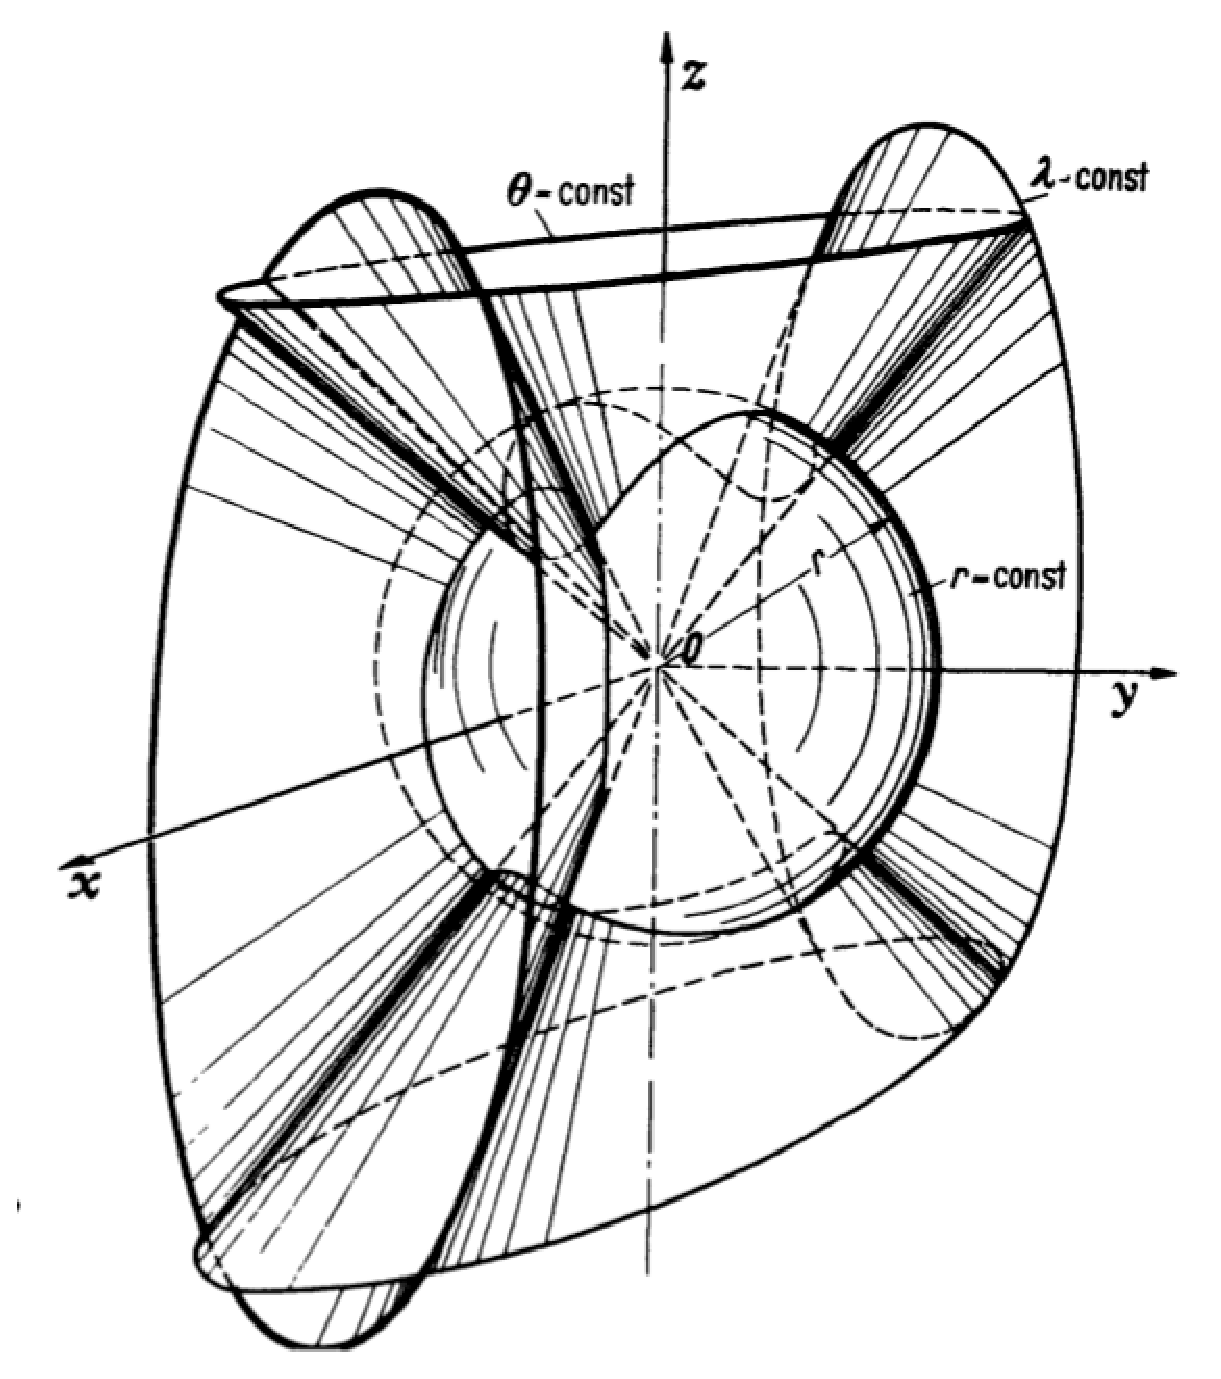
\includegraphics[scale=0.5]{Imagenes/Sistema_Conico.eps}
    \caption{Sistema coordenado cónico.}
\end{figure}

\subsection{Coord. elipsoidales \texorpdfstring{$(\eta, \theta, \lambda)$}{(e, t, l)}.}

Dominio de las coordenadas:
\begin{align*}
c^{2} &< \eta^{2} < \infty, \\
b^{2} &< \theta^{2} < c^{2}, \\
0 &\leq \lambda^{2} < b^{2},
\end{align*}
Con:
\begin{align*}
\eta^{2} > c^{2} > \theta^{2} > b^{2} > \lambda^{2} > 0
\end{align*}

Reglas de transformación:
\begin{align*}
(x)^{2} &= \left( \dfrac{\eta \, \theta \, \lambda}{b \, c} \right)^{2} \\[0.5em]
(y)^{2} &= \dfrac{(\eta^{2} - b^{2})(\theta^{2} - b^{2})(b^{2} - \lambda^{2})}{b^{2}(c^{2} - b^{2})} \\[0.5em]
(z)^{2} &= \dfrac{(\eta^{2} - c^{2}) (c^{2} - \theta^{2})(c^{2} - \lambda^{2})}{c^{2} (c^{2} - b^{2})}
\end{align*}

Factores de escala:
\begin{align*}
(h_{1})^{2} &= \dfrac{(\eta^{2} - \theta^{2})(\eta^{2} - \lambda^{2})}{(\eta^{2} - b^{2})(\eta^{2} - c^{2})} \\[0.5em]
(h_{2})^{2} &= \dfrac{(\theta^{2} - \lambda^{2})(\eta^{2} - \theta^{2})}{(\theta^{2} - b^{2})(c^{2} - \theta^{2})} \\[0.5em]
(h_{3})^{2} &= \dfrac{(\eta^{2} - \lambda^{2})(\theta^{2} - \lambda^{2})}{(b^{2} -  \lambda^{2})(c^{2} - \lambda^{2})}
\end{align*}

\begin{figure}[H]
    \centering
    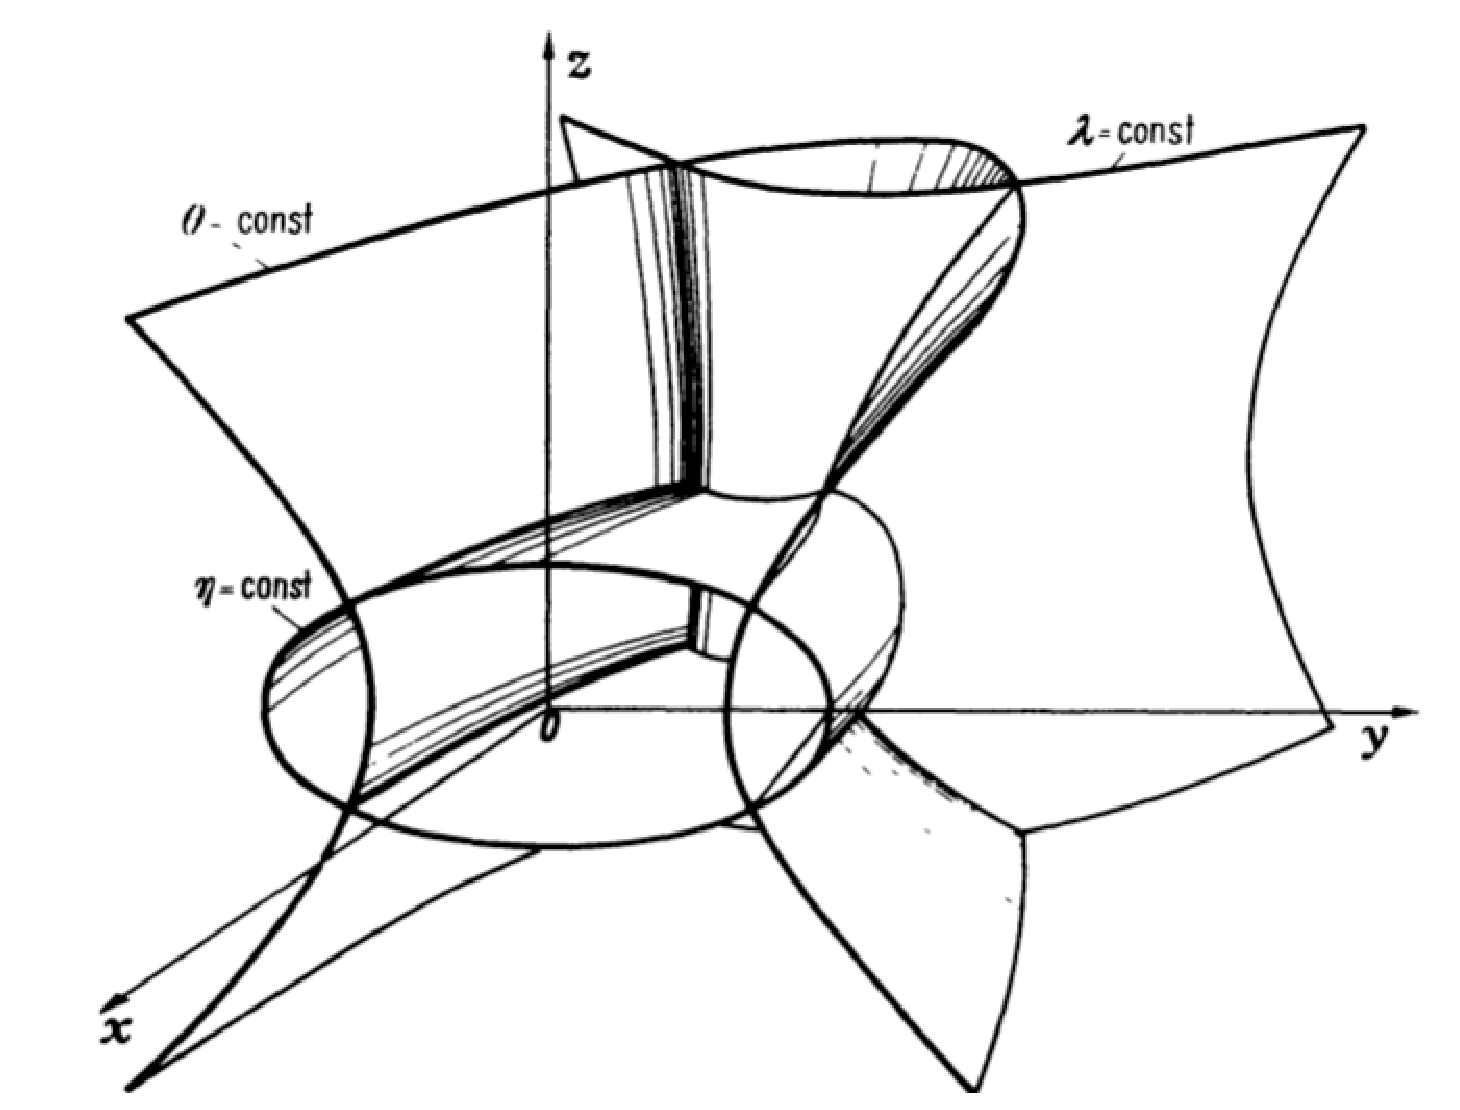
\includegraphics[scale=0.5]{Imagenes/Sistema_Elipsoidal.eps}
    \caption{Sistema coordenado elipsoidal.}
\end{figure}

\subsection{Coord. paraboloides \texorpdfstring{$(\mu, \nu, \lambda)$}{(m, n, l)}.}

Dominio de las coordenadas:
\begin{align*}
b &< \mu < \infty \\
0 &< \nu < c \\
c &< \lambda < b
\end{align*}
Con:
\begin{align*}
\mu > b > \lambda > c > \nu > 0
\end{align*}

Reglas de transformación:
\begin{align*}
(x)^{2} &= \dfrac{4}{(b - c)} \, (\mu - b) \\[0.5em]
(y)^{2} &= \dfrac{4}{(b - c)} \, (\mu - c) \\[0.5em]
z &= \mu + \nu + \lambda - b - c
\end{align*}

Factores de escala:
\begin{align*}
(h_{1})^{2} &= \dfrac{(\mu - \nu)(\mu - \lambda)}{(\mu - b)(\mu - c)} \\[0.5em]
(h_{2})^{2} &= \dfrac{(\mu - \nu)(\lambda - \nu)}{(b - \nu)(c - \nu)} \\[0.5em]
(h_{3})^{2} &= \dfrac{(\lambda - \nu)(\mu - \lambda)}{(b - \lambda)(\lambda - c)}
\end{align*}

\begin{figure}[H]
    \centering
    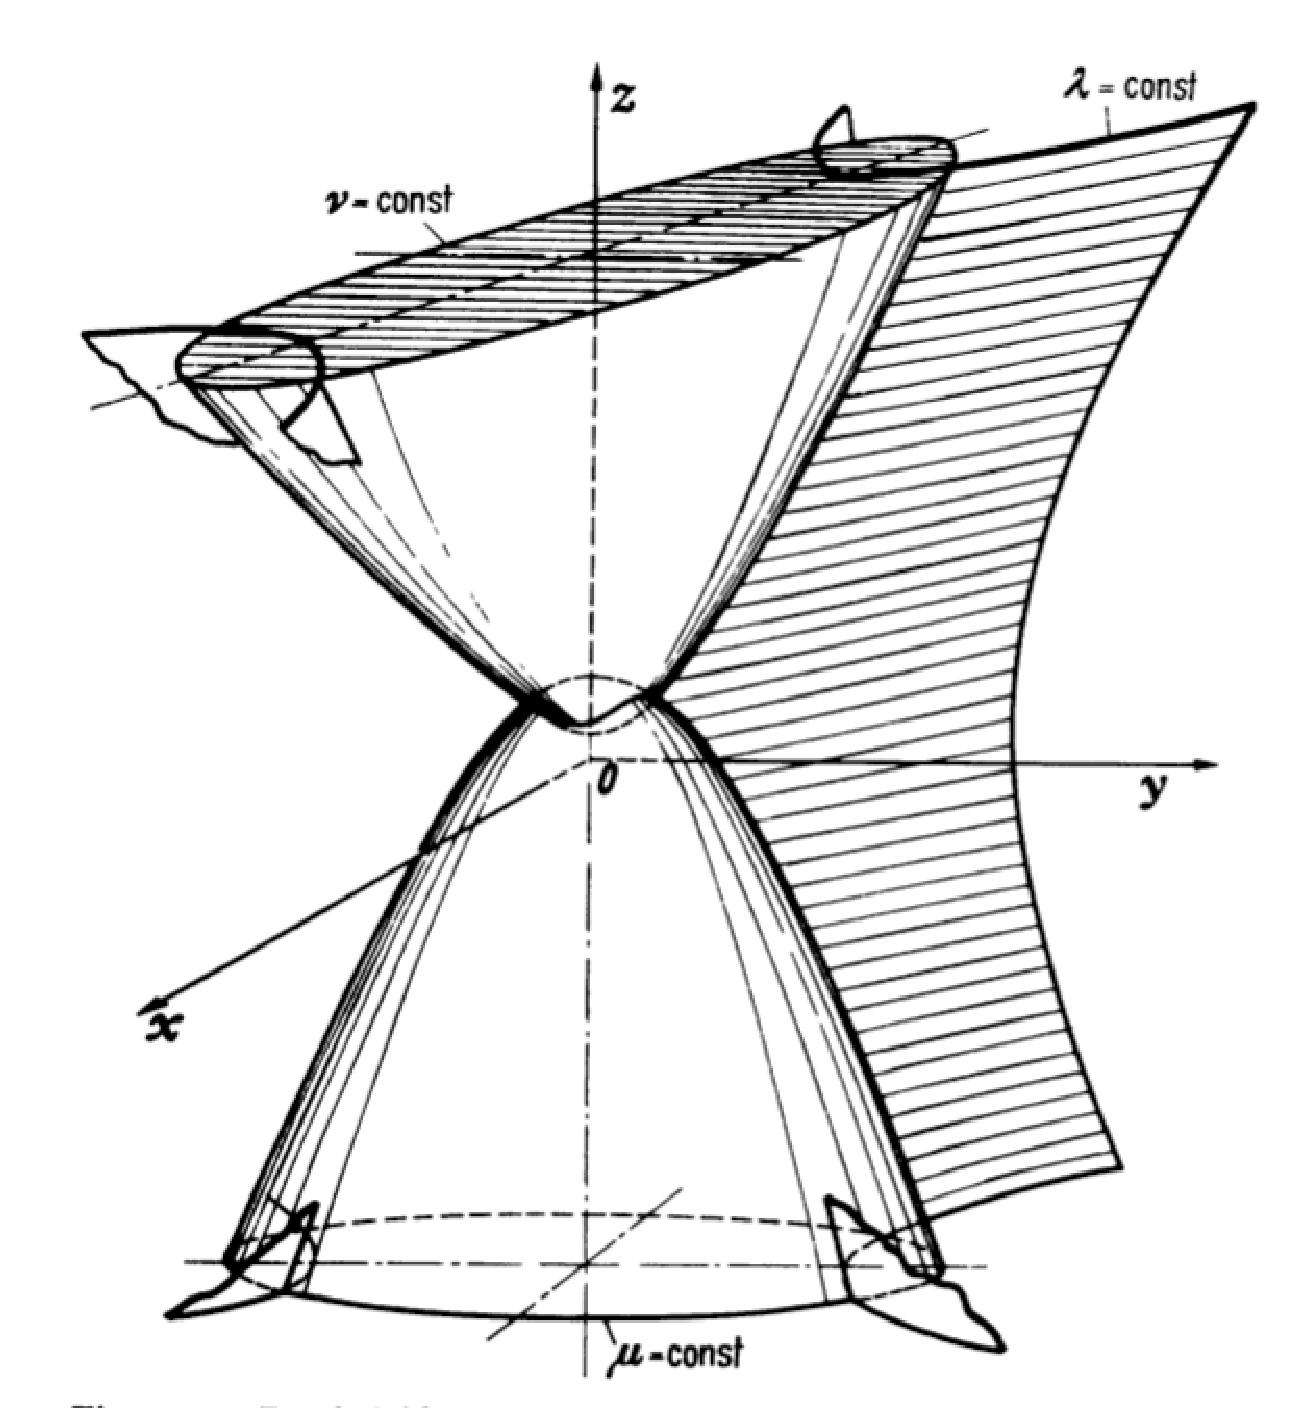
\includegraphics[scale=0.5]{Imagenes/Sistema_Paraboloide.eps}
    \caption{Sistema coordenado paraboloide.}
\end{figure}

\subsection{Coord. cardioide \texorpdfstring{$(\mu, \nu, \psi)$}{(m, n, p)}.}

Dominio de las coordenadas:
\begin{align*}
0 &\leq \mu < \infty \\
0 &\leq \nu < \infty \\
0 &\leq \psi < 2 \, \pi
\end{align*}

Reglas de transformación:
\begin{align*}
x &= \dfrac{\mu \, \nu}{(\mu^{2} + \nu^{2})^{2}} \, \cos \psi \\[0.5em]
y &= \dfrac{\mu \, \nu}{(\mu^{2} + \nu^{2})^{2}} \, \sin \psi \\[0.5em]
z &= \dfrac{1}{2} \, \dfrac{(\mu^{2} - \nu^{2})}{(\mu^{2} + \nu^{2})^{2}}
\end{align*}

Factores de escala:
\begin{align*}
(h_{1})^{2} = (h_{2})^{2} &= \dfrac{1}{(\mu^{2} + \nu^{2})^{3}} \\[0.5em]
(h_{3})^{2} &= \dfrac{\mu^{2} \, \nu^{2}}{(\mu^{2} + \nu^{2})^{4}}
\end{align*}

\begin{figure}[H]
    \centering
    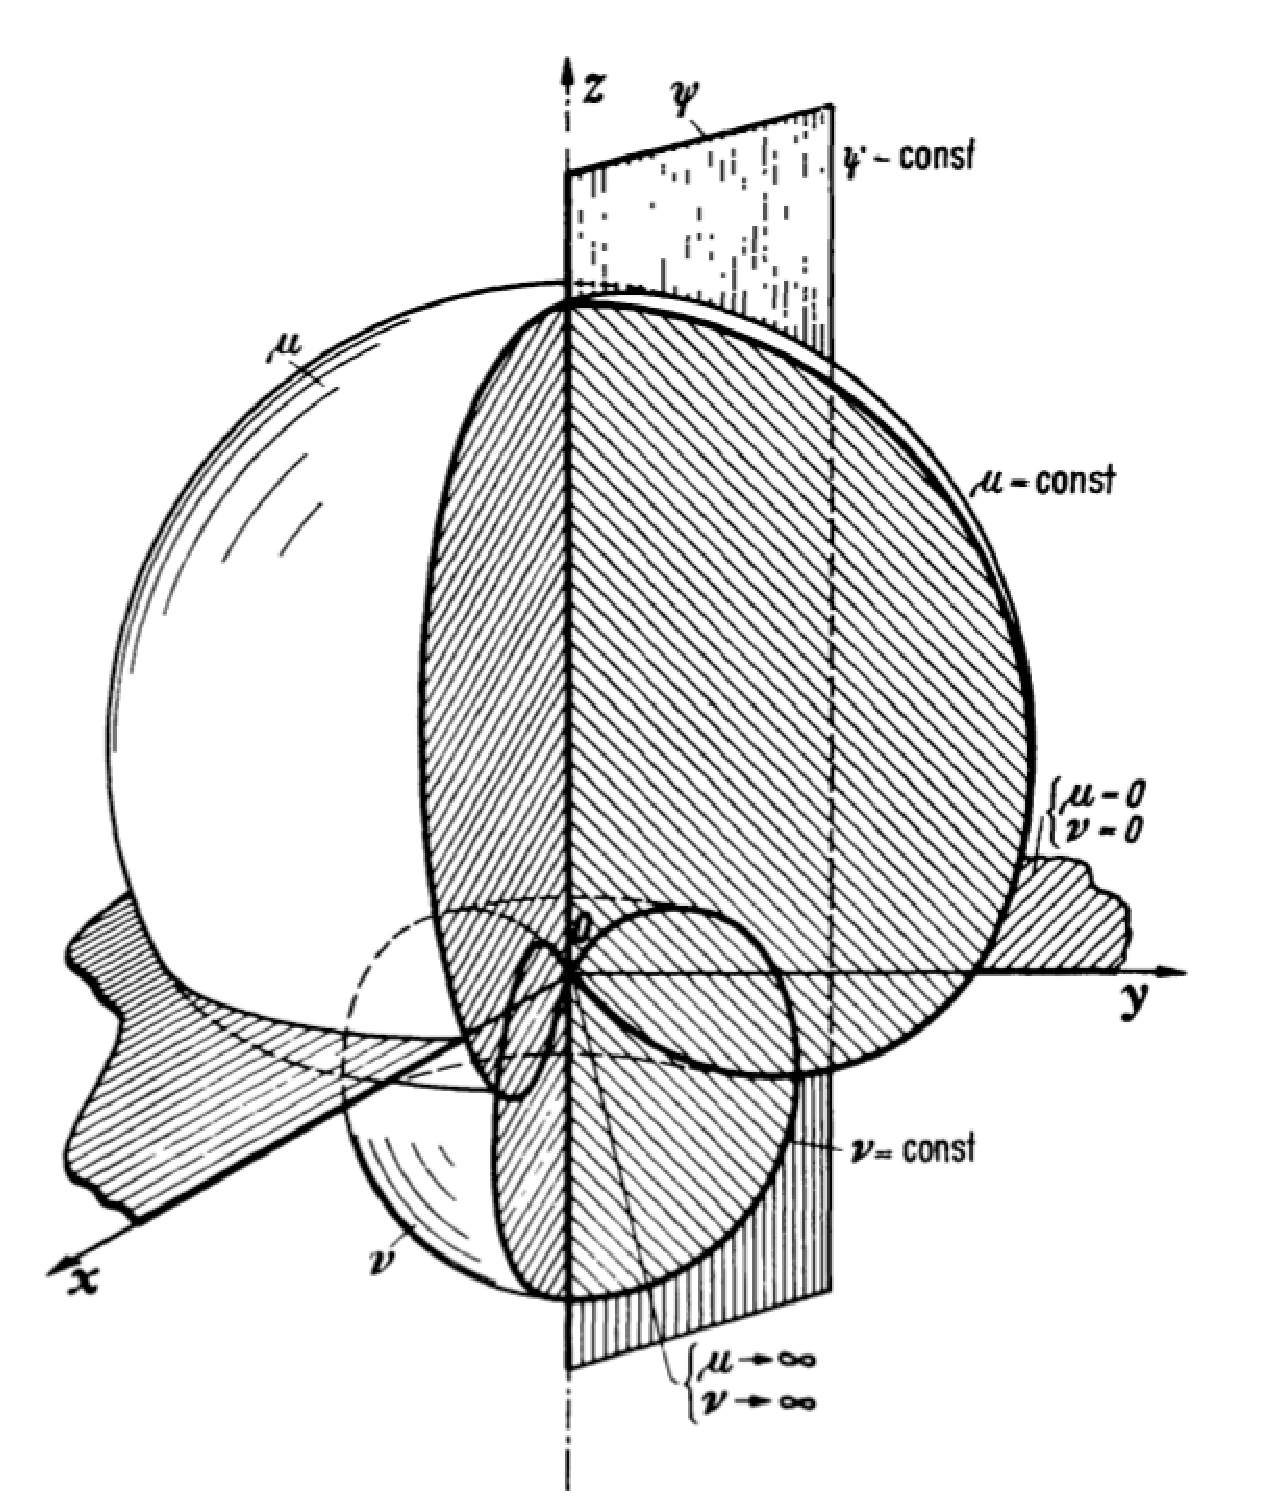
\includegraphics[scale=0.5]{Imagenes/Sistema_Cardioide.eps}
    \caption{Sistema coordenado cardioide.}
\end{figure}

\subsection{Coord. biesféricas \texorpdfstring{$(\eta, \theta, \psi)$}{(e, t, p)}.}

Dominio de las coordenadas:
\begin{align*}
-\infty &< \eta < \infty \\
0 &\leq \theta < \pi \\
0 &\leq \phi < 2\, \pi
\end{align*}

Reglas de transformación:
\begin{align*}
x &= \dfrac{a \, \sin \theta \, \cos \psi}{\cosh \eta - \cos \theta} \\[0.5em]
y &= \dfrac{a \, \sin \theta \, \sin \psi}{\cosh \eta - \cos \theta} \\[0.5em]
z &= \dfrac{a \, \sinh \eta}{\cosh \eta - \cos \theta}
\end{align*}

Factores de escala
\begin{align*}
(h_{1})^{2} = (h_{2})^{2} &= \dfrac{a^{2}}{(\cosh \eta - \cos \theta)^{2}} \\[0.5em]
(h_{3})^{2} &= \dfrac{a^{2} \, \sin^{2} \theta}{(\cosh \eta - \cos \theta)^{2}}
\end{align*}

\begin{figure}[H]
    \centering
    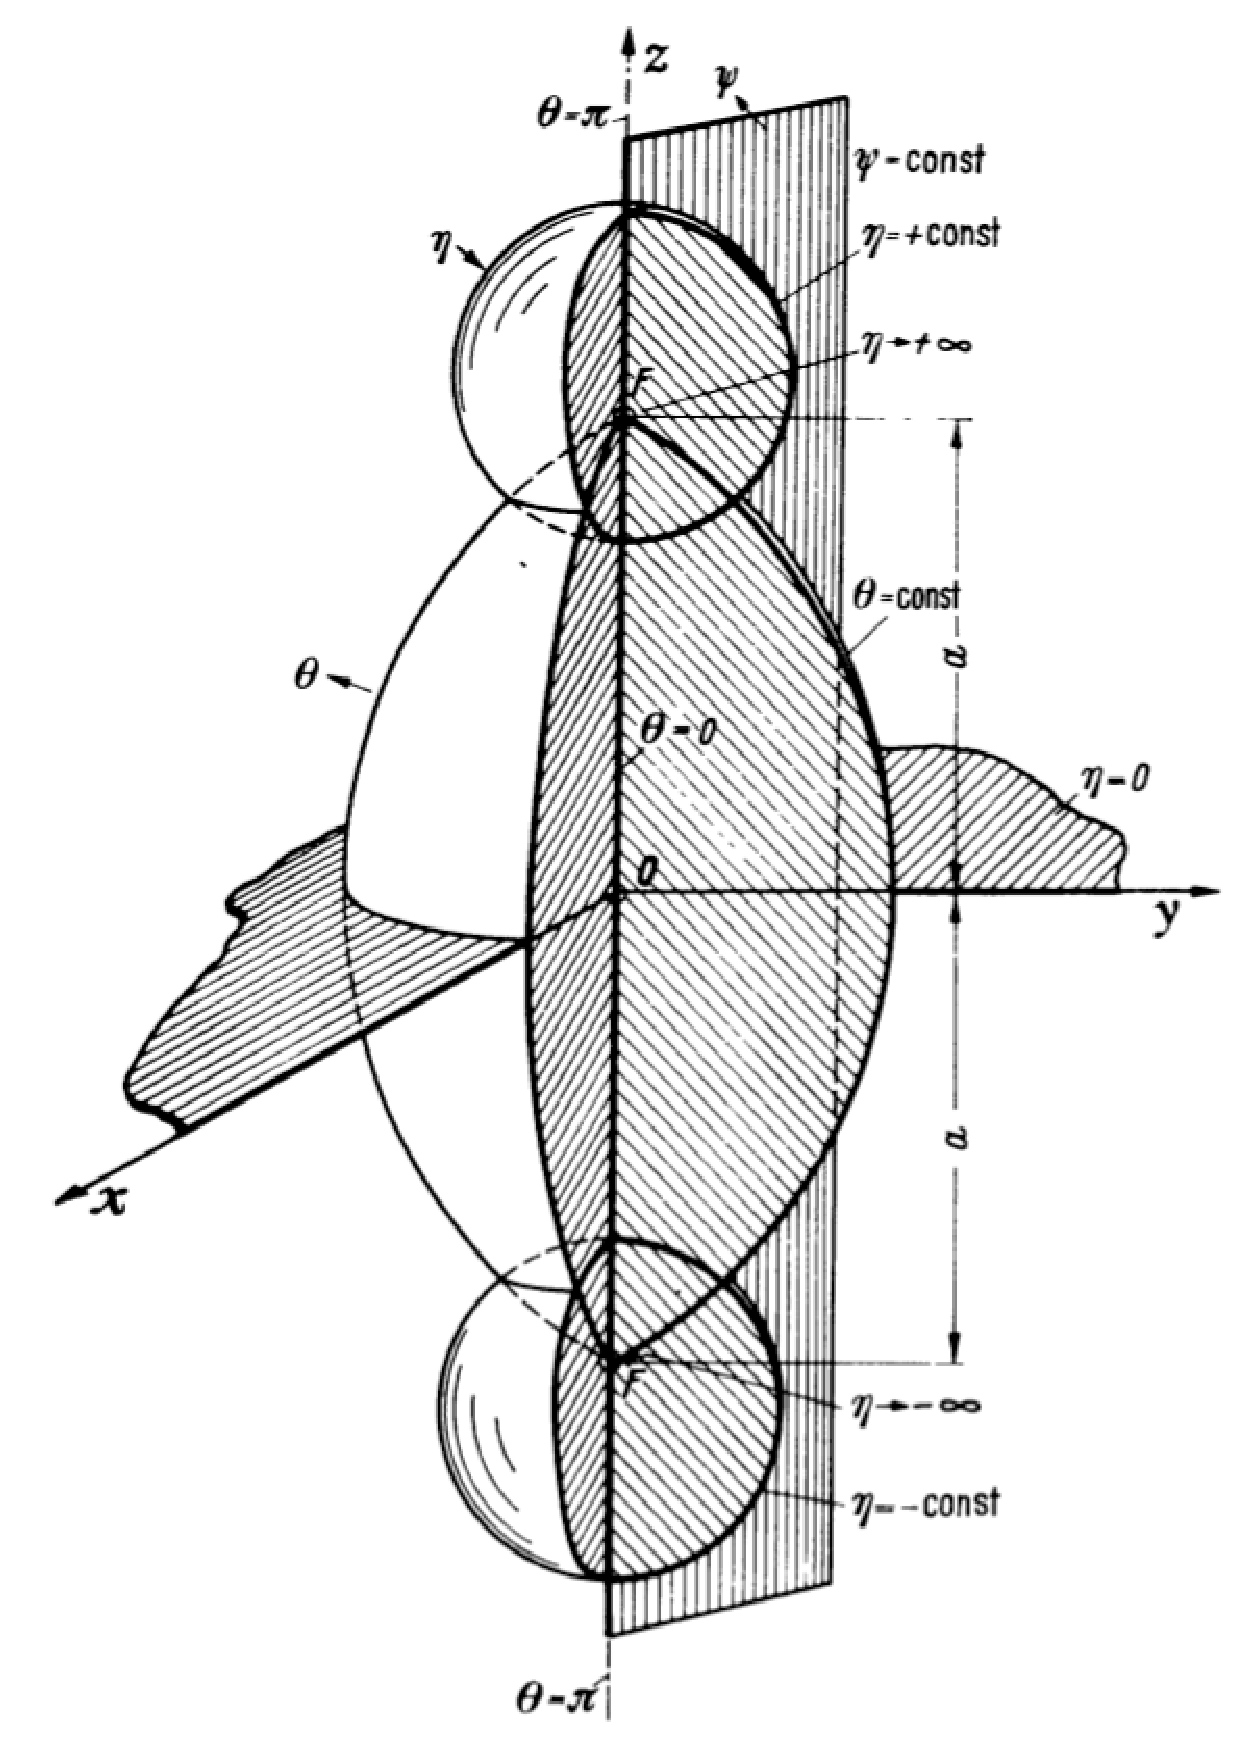
\includegraphics[scale=0.4]{Imagenes/Sistema_Biesferico.eps}
    \caption{Sistema coordenado biesférico.}
\end{figure}

\subsection{Coord. toroidales \texorpdfstring{$(\eta, \theta, \psi)$}{(e, t, p)}.}

Dominio de las coordenadas:
\begin{align*}
0 &\leq \eta < +\infty \\
-\pi &< \theta \leq +\pi \\
0 &\leq \psi < 2\, \pi
\end{align*}

Reglas de transformación:
\begin{align*}
x &= \dfrac{a \, \sinh \eta \, \cos \psi}{\cosh \eta - \cos \theta} \\[0.5em]
y &= \dfrac{a \, \sinh \eta \, \sin \psi}{\cosh \eta - \cos \theta} \\[0.5em]
z &= \dfrac{a \, \sin \theta}{\cosh \eta - \cos \theta}
\end{align*}

Factores de escala:
\begin{align*}
(h_{1})^{2} = (h_{2})^{2} &= \dfrac{a^{2}}{(\cosh \eta - \cos \theta)^{2}} \\[0.5em]
(h_{3})^{2} &= \dfrac{a^{2} \, \sinh^{2} \eta}{(\cosh \eta - \cos \theta)^{2}}
\end{align*}

\begin{figure}[H]
    \centering
    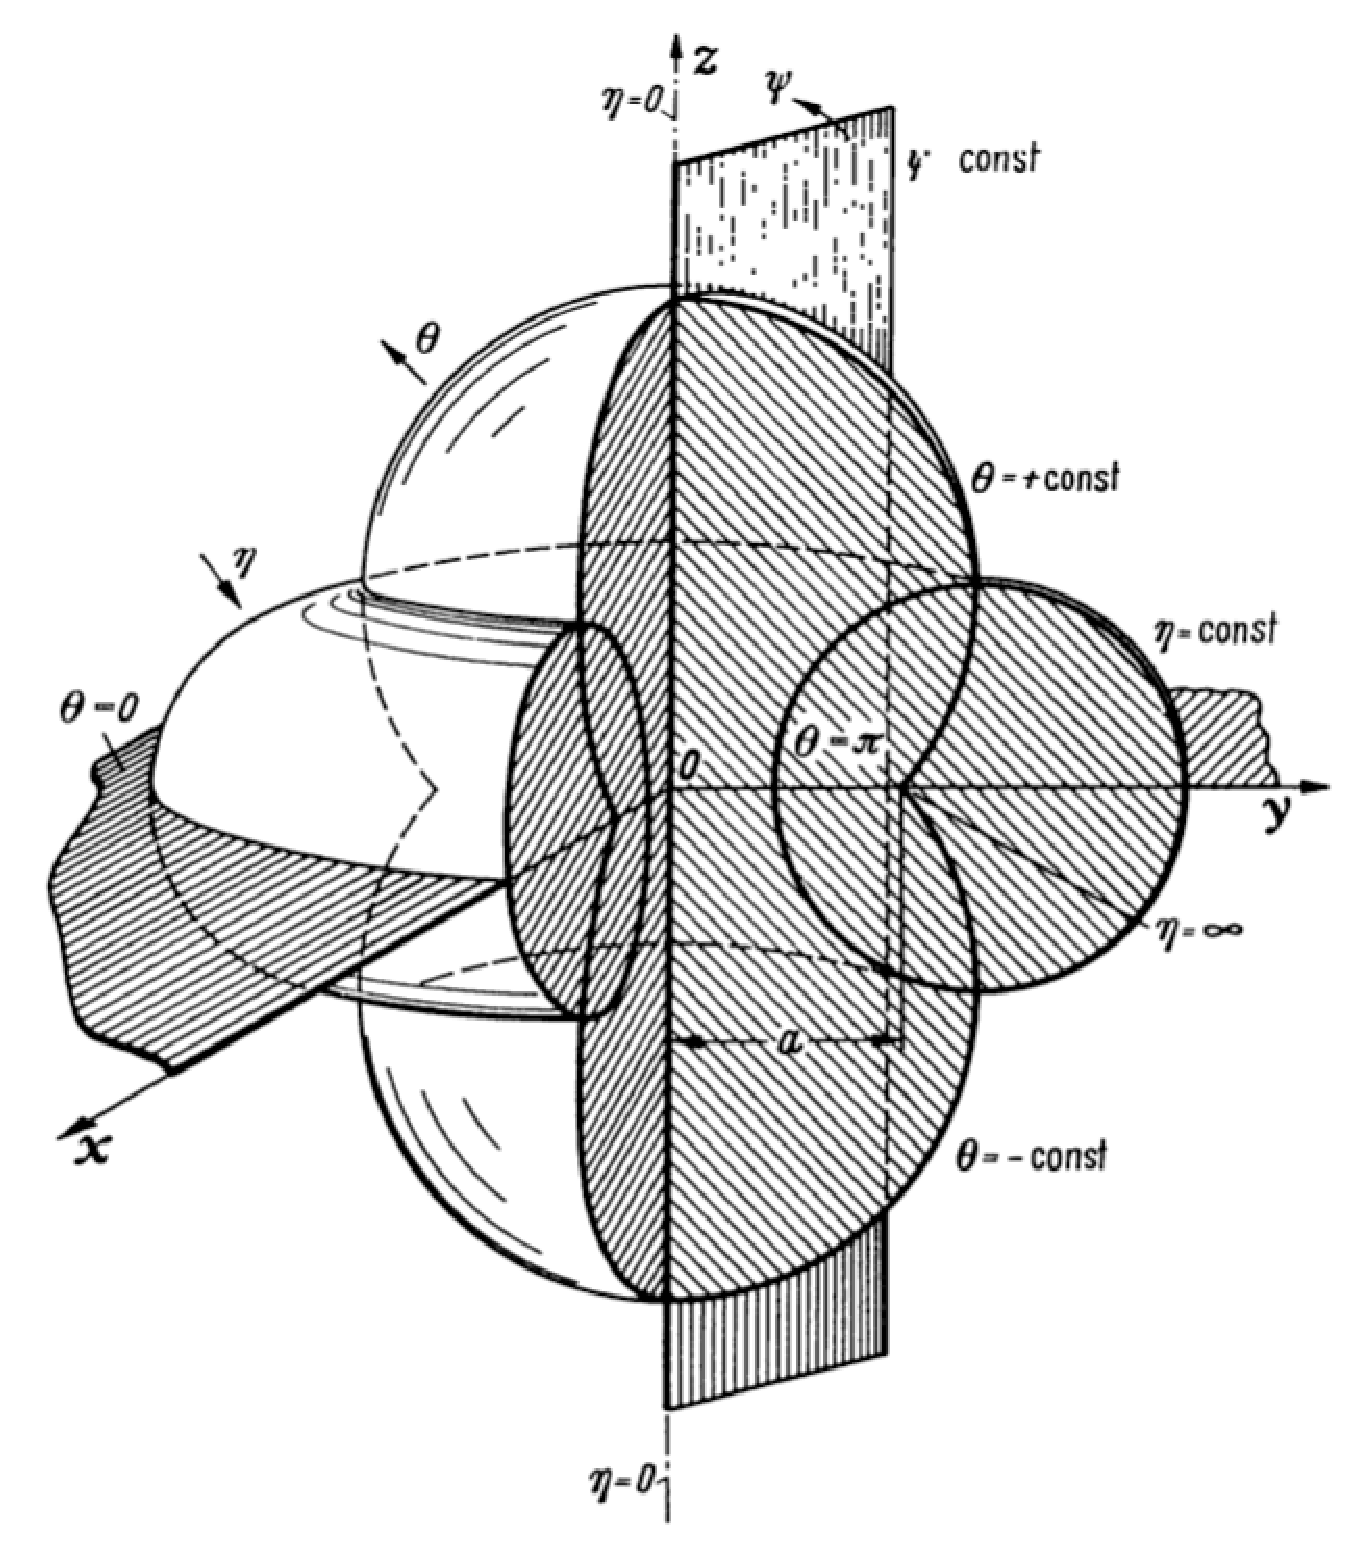
\includegraphics[scale=0.4]{Imagenes/Sistema_Toroidal.eps}
    \caption{Sistema coordenado toroidal.}
\end{figure}

\section{Siguiente paso.}

\subsection{Construcción de otros sistemas}

Una vez que se ha revisado la metodología para construir sistemas curvilíneos, el siguiente paso sería elaborar la descripción de las superficies coordenadas, calcular los factores de escala, obtener los elementos de línea, superficie y volumen, así como los operadores diferenciales.
\par
De esa manera ya podremos expresar la(s) ecuación(es) que definen un problema de la física bajo una geometría en particular. Tendremos que desarrollar estos pasos cuando se nos presente un problema específico.

% \subsection*{Ejercicios a cuenta.}
% Ocupando los siguientes sistemas coordenados\footnote{Deberás de realizar todo el desarrollo correspondiente para los factores de escala necesarios, mientras que podrás ocupar las expresiones de los operadores diferenciales, sin necesidad de repetir el cálculo de los mismos.}, calcula los operadores diferenciales $\grad{\phi}$, $\div{\vb{B}}$, $\curl{\vb{B}}$ y $\laplacian{\phi}$:
% \begin{enumerate}
% \item \textbf{Ejercicio a cuenta (12). } Con el sistema de coordenadas esferoidales prolatas $(\xi, \eta, \phi)$.
% \item \textbf{Ejercicio a cuenta (13). } Con el sistema de coordenadas toroidal $(\eta, \theta, \psi)$.
% \end{enumerate}
\end{document}